% !TeX program = xelatex
% Build from repo root: make -C reports/defense_beamer
% PPTX-inspired editable Beamer. Original and presentation-only vector assets.
\documentclass[aspectratio=169,12pt,t]{beamer}
% White 16:9 style, based on the attached editable PPTX.
\usepackage{fontspec,graphicx,booktabs,array,amsmath,tikz}
\IfFontExistsTF{Aptos}{\setsansfont{Aptos}}{\setsansfont{Helvetica Neue}}
\usefonttheme{professionalfonts}
\pdfstringdefDisableCommands{\def\translate#1{#1}}
\setbeamercolor{normal text}{fg=black,bg=white}
\setbeamercolor{frametitle}{fg=black,bg=white}
\setbeamercolor{structure}{fg=black}
\setbeamerfont{frametitle}{size=\fontsize{19}{23}\selectfont,series=\bfseries}
\setbeamersize{text margin left=9mm,text margin right=9mm}
\setbeamertemplate{navigation symbols}{}
% Bound titles to the text area and reset paragraph alignment explicitly.
% Long titles wrap naturally rather than inheriting body/column alignment.
\setbeamertemplate{frametitle}{%
\vspace{3mm}%
\noindent\begin{minipage}[t]{\textwidth}
\raggedright\usebeamerfont{frametitle}\insertframetitle\par
\end{minipage}\par\vspace{3mm}}
\setbeamertemplate{itemize item}{\small\textbullet}
\setlength{\parindent}{0pt}
\setlength{\parskip}{4pt}
\newif\ifbackup
\setbeamertemplate{footline}{\hspace{9mm}\fontsize{7}{9}\selectfont\ifbackup V\fi\insertframenumber\hfill\vspace{2mm}}
\setbeamertemplate{background}{%
\begin{tikzpicture}[remember picture,overlay]
\node[anchor=south east,inner sep=0pt] at ([xshift=-3mm,yshift=1.5mm]current page.south east){
\includegraphics[width=7mm]{assets/hi-logo.png}};
\end{tikzpicture}}
\graphicspath{{assets/}{../main/figures/}}
\newcommand{\points}{\setlength{\itemsep}{5mm}}
\newcommand{\plainnote}[1]{\par\vspace{2mm}{\small #1\par}}
\newcommand{\originalfigure}[2][6.4cm]{\vspace{-2mm}{\centering\includegraphics[width=\linewidth,height=#1,keepaspectratio]{#2}\par}}
% Full vector artwork with title space intentionally reserved at upper left.
\newcommand{\seasonresult}[3]{%
\begin{frame}[plain]
\begin{tikzpicture}[remember picture,overlay]
\node[anchor=center,inner sep=0pt] at (current page.center){\includegraphics[width=\paperwidth,height=\paperheight,keepaspectratio]{#3}};
\node[anchor=north west,align=left,text width=6.8cm,inner sep=0pt,font=\fontsize{20}{24}\selectfont\bfseries] at ([xshift=8mm,yshift=-5mm]current page.north west){#1};
\node[anchor=north west,align=left,text width=6.8cm,inner sep=0pt,font=\fontsize{11}{14}\selectfont] at ([xshift=8mm,yshift=-18mm]current page.north west){#2};
\node[anchor=south east,inner sep=0pt] at ([xshift=-2mm,yshift=.5mm]current page.south east){
\includegraphics[width=5mm]{assets/hi-logo.png}};
\node[anchor=south west,inner sep=0pt,font=\fontsize{7}{9}\selectfont] at ([xshift=3mm,yshift=1mm]current page.south west){\insertframenumber};
\end{tikzpicture}
\end{frame}}

\hypersetup{pdftitle={Vindur, hitastig og umferðarslys með meiðslum í dreifbýli á Íslandi},pdfauthor={Ásgeir Snær Magnússon}}
\begin{document}

% Main 1: Titill. 1.00 min. Source: Previous main 1
\begin{frame}[plain]
\relax
\vspace{3mm}
{\fontsize{23}{28}\selectfont\bfseries Vindur, hitastig og\\umferðarslys með\\meiðslum í dreifbýli á Íslandi\par}
\vspace{4mm}
2007--2025\par
\vspace{5mm}
\textbf{Ásgeir Snær Magnússon}\par
M.Sc. í hugbúnaðarverkfræði\par
Háskóli Íslands\par
\vspace{4mm}
{\small Leiðbeinandi: Kristján Jónasson\par
Meðleiðbeinandi: Guðmundur Freyr Úlfarsson\par}
\end{frame}

% Main 2: Hvernig tengjast veður og slys?. 1.00 min. Source: Previous main 2
\begin{frame}{Hvernig breytist slysatíðni m.t.t. mismunandi veðurs og umferðar?}
\relax
\begin{enumerate}\points
\item \textbf{Slys miðað við veðurtíðni}\\Eru slysin fleiri en búast mætti við miðað við veðurtíðni?
\item \textbf{Nálguð umferðarleiðrétting}\\Breytist niðurstaðan þegar tekið er tillit til umferðar?
\item \textbf{Slys miðað við áætlaðan akstur}\\Hversu mörg slys verða á milljón VKT?
\end{enumerate}
\end{frame}

% Main 3: Hvaðan koma gögnin?. 0.70 min. Source: Thesis 3.1, source table
\begin{frame}{Hvaðan koma gögnin?}
\relax
\textbf{Samgöngustofa} — slysatími, staðsetning, meiðsli og ökutæki.\par
\textbf{Veðurstofa Íslands} — meðalvindur, vindhviður og hitastig.\par
\textbf{Vegagerðin} — vegkaflar, vegalengdir og umferðartalningar.\par
\textbf{Hagstofa Íslands} — þéttbýlismörk fyrir slys og vegalengdir.\par
\vspace{5mm}
Slys og veður: \textbf{2007--2025}.\par
Daglegar umferðartalningar: \textbf{2019--2024}, á völdum köflum.
\end{frame}

% Main 4: Slys með meiðslum í dreifbýli. 0.60 min. Source: Previous main 3
\begin{frame}{Slys með meiðslum í dreifbýli}
\relax
\originalfigure[5.4cm]{accident_map.png}
{\small 6.414 slys með meiðslum í dreifbýli\par
6.259 þeirra tengd gildri veðurmælingu\par}
\end{frame}

% Main 5: Frá hráum gögnum að greiningu. 1.00 min. Source: Thesis 3.1–3.2
\begin{frame}{Frá hráum gögnum að greiningu}
\relax
{\small\renewcommand{\arraystretch}{1.3}
\begin{tabular}{@{}>{\raggedright\arraybackslash}p{3.3cm}c>{\raggedright\arraybackslash}p{4.0cm}c>{\raggedright\arraybackslash}p{4.2cm}@{}}
\textbf{Gögn} && \textbf{Úrvinnsla} && \textbf{Úttak}\\
Slys og ökutæki & $\to$ & Tengja slys og ökutæki, og velja slys í rannsóknina & $\to$ & Slys með meiðslum í dreifbýli\\
Veðurmælingar & $\to$ & Hreinsa mælingar og reikna veðurtíðni & $\to$ & Gildar mælingar og veðurtíðni\\
Talningar og vegir & $\to$ & Tengja kafla, ár og daga & $\to$ & Áætlaður akstur\\
\end{tabular}\par}
\vspace{4mm}
Tengt eftir tíma, staðsetningu og vegauðkennum.\par
Endurkeyranleg gagnahreinsun og  -niðurstöður.
\end{frame}

% Main 6: Hvaða veðurmælingar eru notaðar?. 0.90 min. Source: Thesis 3.1.2, exact thresholds in V10
\begin{frame}{Hvaða veðurmælingar eru notaðar?}
\relax
\begin{itemize}\points
\item Mælingar sem vantar eða eru utan leyfilegra marka eru útilokaðar.
\item Ósamræmi milli meðalvinds og hviða er síað frá.
\item Langar samfelldar núllraðir eru útilokaðar sem mögulegar mælatruflanir.
\end{itemize}
\vspace{3mm}
\textbf{Aðalgreining slysa og veðurs}\par
Næsta stöð með gilda mælingu innan 20 km frá slysstað og $\pm5$ mínútna.
\end{frame}

% Main 7: Slysafjöldi eftir árum. 0.60 min. Source: Thesis Fig 4.1, annual-counts caption
\begin{frame}{Slysafjöldi eftir árum}
\relax
\originalfigure{annual_accident_counts.pdf}
\end{frame}

% Main 8: Hvenær verða slysin?. 0.90 min. Source: Thesis Fig 3.2; promoted V10
\begin{frame}{Hvenær verða slysin?}
\relax
\begin{tikzpicture}[remember picture,overlay]
\node[anchor=center,inner sep=0pt] at ([yshift=-3.5mm]current page.center){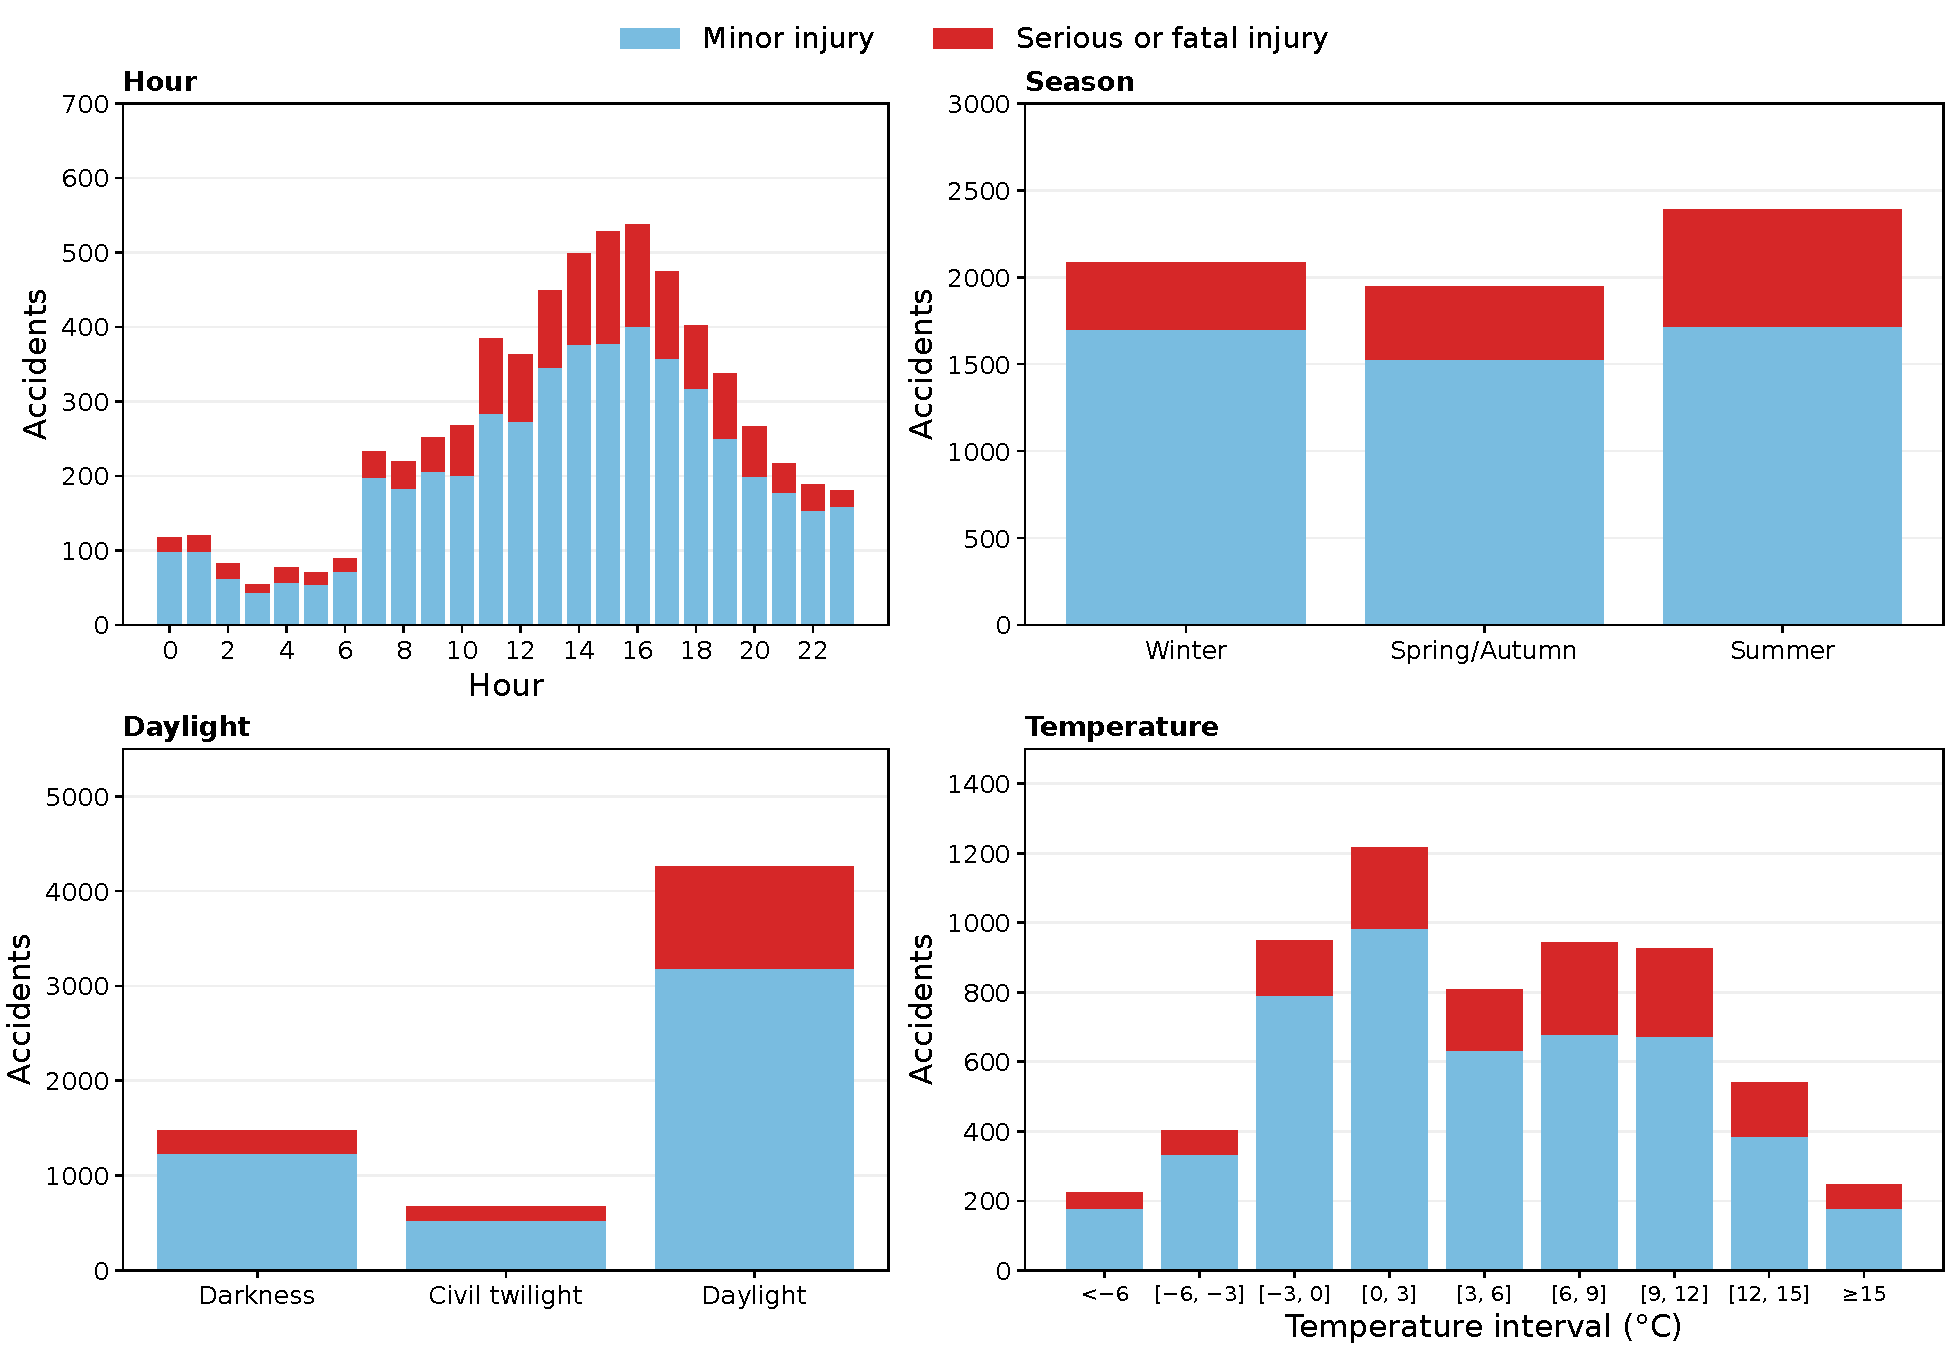
\includegraphics[height=6.65cm,keepaspectratio]{conditions.pdf}};
\node[anchor=center,inner sep=0pt,font=\small] at ([yshift=5mm]current page.south){Slysafjöldi, án leiðréttingar fyrir veðurtíðni eða umferð.};
\end{tikzpicture}
\end{frame}

% Main 9: Hvað ræður væntum slysafjölda?. 1.30 min. Source: Previous main 5
\begin{frame}{Hvað ræður væntum slysafjölda?}
\relax
\setlength{\parskip}{1pt}
\[
\text{Væntur fjöldi}=\text{slysafjöldi}\times\text{veðurtíðni}
\]
Reiknað fyrir hverja veðurstöð og árstíð.\par
\vspace{3mm}
\textbf{Tilbúið skýringardæmi}\par
\renewcommand{\arraystretch}{1.35}
\begin{tabular}{@{}lrr@{}}\toprule
& Staður A & Staður B\\\midrule
Öll slys í hópnum & 100 & 100\\
Tíðni mikils vinds & 10\% & 1\%\\
Vænt slys í miklum vindi & 10 & 1\\\bottomrule
\end{tabular}\par
\vspace{3mm}
Væntir fjöldar eru síðan lagðir saman yfir hópana.
\end{frame}

% Main 10: O/E: skráð slys og væntur fjöldi. 1.20 min. Source: Previous main 6
\begin{frame}{O/E: skráð slys og væntur fjöldi}
\relax
\[
O/E=\frac{\text{skráð slys}}{\text{vænt slys}}
\]
6.259 tengd slys, 2007--2025. Meðalvindur $\geq20$ m/s:\par
{\Large\[\frac{68}{31{,}6}\approx2{,}15\]}
O/E = 1 þegar skráð og vænt slys eru jafnmörg.\par
\vspace{3mm}
{\small Hér er tekið tillit til veðurtíðni, ekki umferðarmagns.\par
2,15 er ekki hlutfallið gagnvart 0--5 m/s.\par}
\end{frame}

% Main 12: Meðalvindur og slys. 1.30 min. Source: Previous main 7
\seasonresult{Meðalvindur og slys}{O/E eftir veðurtíðni}{oe_f.pdf}

% Main 13: Vindhviður og slys. 0.70 min. Source: Previous main 8
\seasonresult{Vindhviður og slys}{O/E eftir veðurtíðni}{oe_fg.pdf}

% Main 14: Hitastig og slys. 0.70 min. Source: Previous main 9
\seasonresult{Hitastig og slys}{O/E eftir veðurtíðni}{oe_temperature.pdf}

% Main 15: Hversu lengi var veðrið í hverju bili?. 0.80 min. Source: src/traffic/daytime_weather.py, daily_vkt.py; thesis3.3.3
\begingroup
% Local title placement: anchor to the physical page, not frame text flow.
% The invisible title keeps the existing title-box height and body position.
\setbeamertemplate{frametitle}{%
\vspace{3mm}%
\noindent\begin{minipage}[t]{\textwidth}
\raggedright\usebeamerfont{frametitle}%
\begin{tikzpicture}[remember picture,overlay]
\node[anchor=base west,inner sep=0pt,align=left,
      text width=\dimexpr\paperwidth-18mm\relax,
      font=\usebeamerfont{frametitle}]
      at ([xshift=9mm,yshift=-11mm]current page.north west)
      {\insertframetitle};
\end{tikzpicture}%
\phantom{\insertframetitle}\par
\end{minipage}\par\vspace{3mm}}
\begin{frame}{Hversu lengi var veðrið í hverju bili?}
\relax
\setlength{\parskip}{3pt}
{\large\[
q=\frac{\text{mínútur með gildum mælingum í veðurbilinu}}
       {\text{1.020 mínútur frá kl. 07 til 24}}
\]}
\textbf{Dæmi:} 102 mínútur í miklum vindi $\to q=0{,}10$.\par
\vspace{3mm}
Þá fara 10\% af bæði mældri og væntri sólarhringsumferð í það vindbil.\par
\vspace{3mm}
Tími án gildra veðurmælinga fær enga úthlutun.\par
\vspace{3mm}
Þetta er áætluð skipting. Við vitum ekki hversu mikil umferð var á þessum mínútum.
\end{frame}
\endgroup

% Main 16: Umferð í ólíku veðri. 1.30 min. Source: Thesis 3.3.3; src/traffic/daily_vkt.py add_expected_daily_traffic and traffic_response
\begin{frame}{Umferð í ólíku veðri}
\relax
\setlength{\parskip}{2pt}
\setlength{\abovedisplayskip}{6pt}
\setlength{\belowdisplayskip}{6pt}
{\Large\setlength{\abovedisplayskip}{4pt}\setlength{\belowdisplayskip}{4pt}\[
r_j=\frac{\sum_{c,d}C_{cd}\,q_{cdj}}{\sum_{c,d}B_{cd}\,q_{cdj}}
\]}
$C$: mæld og $B$: vænt sólarhringsumferð, 2019--2024.\par
$B$ er meðaltal jákvæðra talninga á sama kafla, ári, mánuði og vikudegi.\par
\vspace{2mm}
$c$: teljarakafli. $d$: dagur. $j$: veðurbil.\par
$q$: hlutfall tímans frá kl. 07--24 með gildum mælingum í veðurbilinu.\par
\vspace{3mm}
$r_j=0{,}8$: mæld umferð sem fellur í veðurbilið samkvæmt skiptingunni er 20\% minni en sú vænta.\par
\end{frame}

% Main 17: Umferð eftir veðri. 0.45 min. Source: Previous main 11
\begin{frame}{Umferð eftir veðri}
\relax
\originalfigure[6.6cm]{traffic_response.pdf}
\end{frame}

% Main 18: Sami slysafjöldi, nýr væntur fjöldi. 0.85 min. Source: Previous main 12
\begin{frame}{Sami slysafjöldi, nýr væntur fjöldi}
\relax
Veðurhlutföll eru margfölduð með umferðarhlutföllum\par
og endurreiknuð í 100\% við hverja stöð og árstíð.\par
\vspace{4mm}
\renewcommand{\arraystretch}{1.35}
\begin{tabular}{@{}lrr@{}}\toprule
Meðalvindur $\geq20$ m/s & O/E & Leiðrétt O/E\\\midrule
Skráður slysafjöldi & 68 & 68\\
Væntur slysafjöldi & 31,6 & 25,1\\
Hlutfall & 2,15 & 2,71\\\bottomrule
\end{tabular}\par
\vspace{4mm}
{\small Nálguð leiðrétting frá 2019--2024 er notuð fyrir 2007--2025.\par}
\end{frame}

% Main 19: Meðalvindur: fyrir og eftir leiðréttingu. 0.50 min. Source: Previous main 13
\begin{frame}{Meðalvindur: fyrir og eftir leiðréttingu}
\relax
\originalfigure{weather_oe_traffic_corrected_f.pdf}
\end{frame}

% Main 20: Vindhviður: fyrir og eftir leiðréttingu. 0.40 min. Source: Previous main 14
\begin{frame}{Vindhviður: fyrir og eftir leiðréttingu}
\relax
\originalfigure{weather_oe_traffic_corrected_fg.pdf}
\end{frame}

% Main 21: Hitastig: fyrir og eftir leiðréttingu. 0.40 min. Source: Previous main 15
\begin{frame}{Hitastig: fyrir og eftir leiðréttingu}
\relax
\originalfigure{weather_oe_traffic_corrected_temperature.pdf}
\end{frame}

% Main 22: Hvaða slys komast í VKT-greininguna?. 0.80 min. Source: Thesis 3.3.4, Table4.1; promoted V6 summary
\begin{frame}{Hvaða slys komast í VKT-greininguna?}
\relax
\textbf{2019--2024}\par
\vspace{3mm}
\begin{tabular}{@{}rl@{}}
\textbf{1.863} & slys með meiðslum í dreifbýli\\[3mm]
$\downarrow$ & \\
\textbf{869} & á vegum með teljarakafla fyrir viðkomandi ár\\[3mm]
$\downarrow$ & \\
\textbf{694} & uppfylla öll lokaskilyrði\\
\end{tabular}\par
\vspace{4mm}
Staðsetning á kafla, tími kl. 07--24, gilt veður og dagleg talning.\par
{\small Hér er 20 km veðurfjarlægð mæld frá teljarakafla, ekki slysstað.\par}
\end{frame}

% Main 23: Hvernig er akstur áætlaður?. 0.85 min. Source: Previous main 16
\begin{frame}{Hvernig er akstur áætlaður?}
\relax
\[
\begin{aligned}
\text{Áætlaður akstur í dreifbýli} &= \text{sólarhringstalning}\\
&\quad\times\text{lengd kaflans utan þéttbýlis}
\end{aligned}
\]
\vspace{3mm}
VKT = áætlaður heildarfjöldi ekinna km í þessari greiningu.\par
\vspace{4mm}
\[
10\ \text{ökutæki}\times1\ \text{km}=10\ \text{eknir km}
\]
\vspace{4mm}
Gert er ráð fyrir að talningin lýsi umferð um dreifbýlishluta kaflans.\par
{\small Slys og veður kl. 07--24, en umferðartalningar ná yfir allan sólarhringinn.\par}
\end{frame}

% Main 24: Skipting aksturs eftir veðri. 1.20 min. Source: Thesis3.3.4, monthly allocation
\begin{frame}{Skipting aksturs eftir veðri}
\relax
\begin{columns}[t,onlytextwidth]
\begin{column}{.45\textwidth}\textbf{Slys}\par
Flokkast eftir veðrinu þegar slysið varð.\end{column}
\begin{column}{.51\textwidth}\textbf{Áætlaður akstur}\par
Skiptingin fylgir langtímaveðurtíðni hvers mánaðar við stöðina.\end{column}
\end{columns}
\vspace{5mm}
Veðurtíðni kl. 07--24, sameinuð yfir 2007--2025.\par
Daglegar umferðartalningar eru áfram ólíkar milli daga.\par
Dagar án slysa telja líka með í akstrinum.\par
\vspace{4mm}
Skiptingin endurskapar ekki raunverulegan akstur í veðrinu hvern dag.
\par
\[
\text{Slysatíðni}=\frac{\text{slys í veðurbili}}{\text{áætlað VKT í veðurbili}}\times10^6
\]
\end{frame}

% Main 26: Meðalvindur og slys. 0.85 min. Source: Previous main 18
\seasonresult{Meðalvindur og slys}{Slys / milljón áætlaðra VKT}{vkt_f.pdf}

% Main 27: Vindhviður og slys. 0.65 min. Source: Previous main 19
\seasonresult{Vindhviður og slys}{Slys / milljón áætlaðra VKT}{vkt_fg.pdf}

% Main 28: Hitastig og slys. 0.80 min. Source: Previous main 20
\seasonresult{Hitastig og slys}{Slys / milljón áætlaðra VKT}{vkt_temperature.pdf}

% Main 29: Er vindmynstrið það sama við öll hitastig?. 1.30 min. Source: Previous main 21
\begin{frame}{Er vindmynstrið það sama við öll hitastig?}
\relax
\begin{tikzpicture}[remember picture,overlay]
\node[anchor=north west,inner sep=0pt,text width=\textwidth,font=\small] at ([xshift=9mm,yshift=-13mm]current page.north west){O/E miðað við sameiginlega tíðni vinds og hitastigs · 2007--2025};
\node[anchor=center,inner sep=0pt] at ([yshift=-6.5mm]current page.center){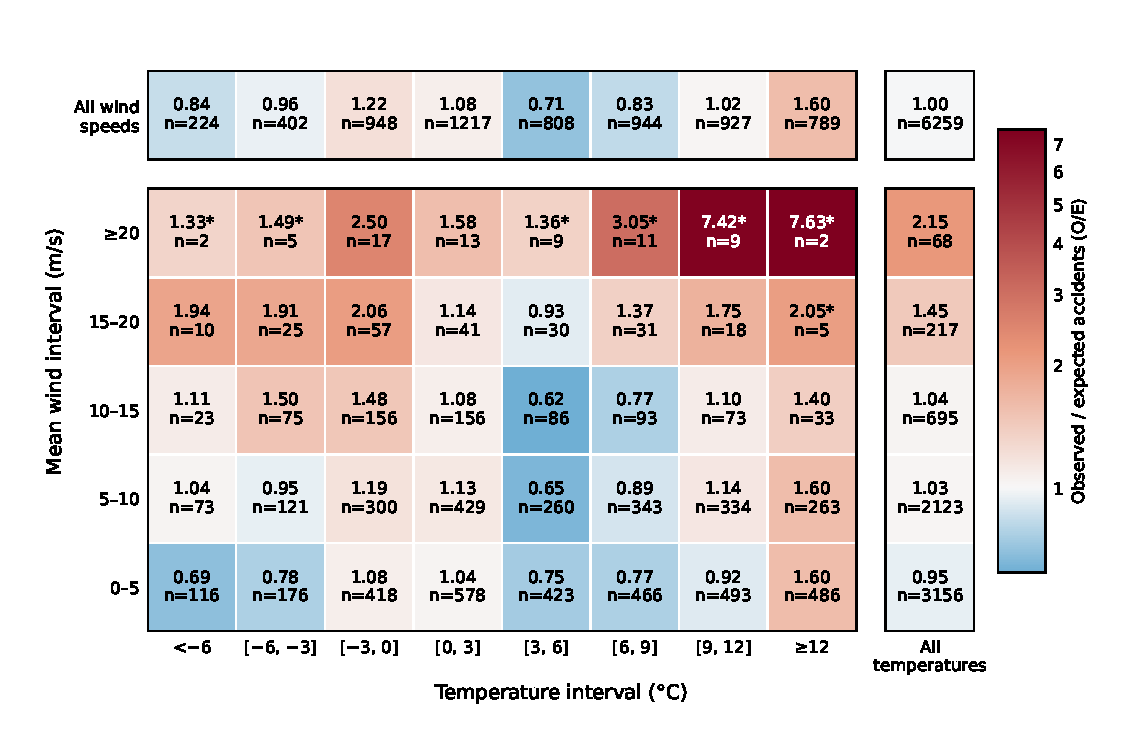
\includegraphics[height=6.1cm,keepaspectratio]{joint_wind_temperature_detail.pdf}};
\node[anchor=south west,inner sep=0pt,font=\footnotesize] at ([xshift=9mm,yshift=4mm]current page.south west){* Færri en 10 skráð slys eða færri en 5 vænt slys, ekki marktækni.};
\end{tikzpicture}
\end{frame}

% Main 30: Samanburður aðferðanna. 1.00 min. Source: Previous main 22
\begin{frame}{Samanburður aðferðanna}
\relax
{\small Hlutfall efsta bils og 0--5 m/s innan hverrar aðferðar.\par}
\vspace{3mm}
\renewcommand{\arraystretch}{1.45}
\begin{tabular}{@{}lrr@{}}\toprule
& \shortstack{Vindur\\$\geq20$ m/s} & \shortstack{Hviður\\$\geq30$ m/s}\\\midrule
O/E & 2,28 & 3,73\\
Umferðarleiðrétt O/E & 2,91 & 4,75\\
Slysatíðni miðað við VKT & 5,83 & 7,78\\\bottomrule
\end{tabular}\par
\vspace{5mm}
{\small O/E fyrir og eftir leiðréttingu byggist á sömu slysum.\par
VKT notar minna úrtak og áætlaðan akstur.\par}
\end{frame}

% Main 31: Hvers vegna eru VKT-hlutföllin stærri?. 1.00 min. Source: Thesis4.4.4; promoted V8 essential explanation
\begin{frame}{Hvers vegna eru VKT-hlutföllin stærri?}
\relax
Akstur í miklum vindi og litlum vindi getur farið fram \textbf{á ólíkum vegköflum og tímabilum}.\par
\vspace{3mm}
\begin{itemize}\points
\item Þegar samanburðurinn var gerður \textbf{innan sama vegkafla, árs og árstíðar} urðu hlutföllin lægri.
\item \textbf{Hluti munarins tengist því hvar og hvenær er ekið}, ekki aðeins vindhraðanum.
\end{itemize}
\vspace{3mm}
\textbf{Hærra hlutfall þýðir ekki sjálfkrafa nákvæmara mat.}
\end{frame}

% Main 32: Helstu takmarkanir. 1.00 min. Source: Previous main 23
\begin{frame}{Helstu takmarkanir}
\relax
\begin{itemize}\points
\item \textbf{Akstur:} Daglegar talningar á hluta vegakerfisins. Skipting aksturs eftir veðri er áætluð.
\item \textbf{Veður:} Mæling við stöð getur verið ólík veðrinu á slysstað.
\item \textbf{Óvissa:} Fá slys í sumum veðurbilum. Öryggisbil eru ekki birt.
\end{itemize}
\vspace{3mm}
\textbf{Niðurstöðurnar sýna tengsl, en staðfesta hvorki orsakasamband né hegðun ökumanna.}
\end{frame}

% Main 33: Næstu skref. 0.70 min. Source: Previous main 24
\begin{frame}{Næstu skref}
\relax
\begin{itemize}\points
\item \textbf{Nákvæmari umferðargögn:} Talningar eftir klukkustundum, talningar á fleiri vegum, svo akstur og veður séu borin saman yfir sama tímabil.
\item \textbf{Aðstæður á vegi:} Tengja slysin við hálku, skyggni og vindátt miðað við stefnu vegar, til að skoða hliðarvind.
\item \textbf{Viðbrögð við veðri:} Nota upplýsingar um hraða og lokanir til að greina betur hvort fólk hægir á sér, frestar ferðum eða kemst ekki leiða sinna.
\item \textbf{Ólíkar tegundir slysa:} Skoða hvort vindmynstrið sé sérstaklega áberandi í útafakstri, veltum eða hjá ákveðnum ökutækjaflokkum.
\end{itemize}
\end{frame}

% Continuation: retain readable text size for all approved next steps.
\begin{frame}{Næstu skref}
\begin{itemize}\points
\item \textbf{Traustari samanburður:} Nota sama slysasafn í greiningunum, reikna öryggisbil og kanna áhrif þess að breyta veðurbilum og skilyrðum.
\item \textbf{Skoða einstaka vegi nánar:} Greina hvar slysin safnast saman og hvort mynstur eftir veðri, árstíð og tegund slyss sé ólíkt milli sambærilegra vegkafla.
\item \textbf{Skoða vind og hitastig saman með tölfræðilíkani:} Meta hvort samband vinds og slysa breytist eftir hitastigi, með óvissumati og nægilegum fjölda slysa.
\end{itemize}
\end{frame}

% Main 34: Helstu niðurstöður. 1.00 min. Source: Thesis4.2–4.4, conclusion
\begin{frame}{Helstu niðurstöður}
\relax
\begin{itemize}\points
\item \textbf{Vindur:} Fleiri slys urðu í miklum vindi en búast mátti við miðað við vindtíðni.
\item \textbf{Umferð:} Umferðarleiðréttingin hækkaði O/E í mesta vindinum. Slysatíðni miðað við áætlaðan akstur var einnig hærri í mesta vindinum.
\item \textbf{Hitastig:} O/E var hækkað rétt undir frostmarki og við $\geq12^{\circ}$C. Slysatíðni miðað við áætlaðan akstur var hæst í kulda, lægst við 9--12$^{\circ}$C og hækkaði aftur við $\geq12^{\circ}$C.
\end{itemize}
\end{frame}

\appendix
\backuptrue
\setcounter{framenumber}{0}

% Backup V1
\begin{frame}{Gögn og heimildir}
\relax
\begin{itemize}
\setlength{\itemsep}{1mm}
\item \textbf{Samgöngustofa:} Slysa- og ökutækjaskrá.
\item \textbf{Veðurstofa Íslands:} Veðurmælingar.
\item \textbf{Vegagerðin:} Umferðartalningar, vegkaflar og vegkaflalengdir.
\item \textbf{Hagstofa Íslands:} Þéttbýlismörk.
\end{itemize}
\vspace{2mm}
\textbf{Kynningin byggist á meistararitgerð minni:}\par
{\small Ásgeir Snær Magnússon (2026).\par
\emph{Wind, Temperature, and Rural Injury Accidents in Iceland.}\par
Meistararitgerð í hugbúnaðarverkfræði, Háskóli Íslands.\par
\vspace{2mm}
Myndir og niðurstöður eru úr ritgerðinni. Þar er einnig að finna ítarlega heimildaskrá.\par}
\end{frame}

% Backup V2
\begin{frame}{O/E og nálguð umferðarleiðrétting}
\relax
\setlength{\parskip}{2pt}
\relax
\[
 R_j=\frac{O_j}{\sum_g A_g p_{jg}}
 \qquad
 R_j^{*}=\frac{O_j}{\sum_g A_g p^{*}_{jg}}
\]
\[
 p_{jg}=\frac{T_{jg}}{T_g}
 \qquad
 p^{*}_{jg}=\frac{p_{jg}r_j}{\sum_h p_{hg}r_h}
\]
\par\vspace{2mm}
{\small
$R_j$ og $R_j^*$: O/E fyrir og eftir leiðréttingu.\par
$O_j$: skráð slys í veðurbili $j$.\par
$g$: stöð og árstíð. $A_g$: slysafjöldi í þeim hópi.\par
$T_{jg}/T_g$: hlutfall gildra veðurmælinga í bilinu.\par
$r_j$: úthlutuð mæld umferð / úthlutuð vænt umferð.\par
$h$: öll veðurbil í summunni sem staðlar vægin.\par}
\end{frame}

% Backup V3
\begin{frame}{Hvernig er umferðarleiðréttingin nálguð?}
\relax
\begin{itemize}\points
\item Vænt dagleg umferð er meðaltal á sama kafla, ári, mánuði og vikudegi. Aðeins jákvæðar talningar eru notaðar.
\item Mældri og væntri sólarhringsumferð er skipt eftir veðurtíma kl. 07--24 á viðkomandi degi.
\item Hlutfall mældrar og væntrar umferðar endurvigtar veðurtíðnina. Viðbragð 2019--2024 er yfirfært á 2007--2025.
\end{itemize}
\plainnote{Þetta eru ekki mælingar á umferð eftir klukkustundum.}
\end{frame}

% Backup V4
\begin{frame}{Áætlaður akstur og slysatíðni}
\relax
\setlength{\parskip}{2pt}
\relax
\[
 \widehat V_{cdb}=C_{cd}L_{c,y(d)}p_{s(c),m(d),b}
 \qquad
 R_b=\frac{O_b}{\sum_{c,d}\widehat V_{cdb}}\,10^6
\]
\par\vspace{1mm}
{\small
$c$: vegkafli með teljara. $d$: dagur. $b$: veðurbil.\par
$C_{cd}$: sólarhringstalning. $L_{c,y(d)}$: lengd dreifbýlishluta kafla á viðkomandi ári.\par
$s(c)$: úthlutuð veðurstöð. $m(d)$: almanaksmánuður.\par
$p_{s(c),m(d),b}$: veðurtíðni kl. 07--24, sameinuð yfir 2007--2025.\par
$\widehat V_{cdb}$: áætlaður akstur í veðurbili $b$, á kafla $c$, á degi $d$.\par
$O_b$: slysafjöldi flokkaður eftir veðri við slysið.\par
$R_b$: slys á milljón áætlaðra ökutækjakílómetra.\par}
{\footnotesize Gert er ráð fyrir að talningin lýsi umferð um dreifbýlishluta vegkaflans.\par}
\end{frame}

% Backup V5
\begin{frame}{Fjarlægð og þekja veðurtengingar}
\relax
{\centering\renewcommand{\arraystretch}{1.4}
\begin{tabular}{@{}rrr@{}}\toprule
Hámarksfjarlægð & Tengd slys & Hlutfall\\\midrule
5 km & 3.060 & 47,7\%\\
10 km & 5.098 & 79,5\%\\
20 km & 6.259 & 97,6\%\\
30 km & 6.402 & 99,8\%\\\bottomrule
\end{tabular}\par}
\plainnote{20 km vegur saman nálægð og þekju.\par
Veðrið getur verið ólíkt við stöð og á slysstað.\par
Þetta er samanburður á þekju, ekki næmnigreining á vindtengslum.}
\end{frame}

% Backup V6
\begin{frame}{Val slysa fyrir mat á slysatíðni}
\relax
{\centering\renewcommand{\arraystretch}{1.25}
\begin{tabular}{@{}lr@{}}
\toprule
Slys með meiðslum, 2007--2025 & 17.045\\
Árin 2019--2024 & 5.196\\
Í dreifbýli & 1.863\\
Vegkafli með teljara fyrir veg og ár & 869\\
Staðsett á vegkafla & 848\\
Kl. 07--24 & 781\\
Gilt vind- og hviðugildi & 777\\
Með daglegri umferðartalningu & 694\\
\bottomrule
\end{tabular}\par}
\plainnote{Veður innan 20 km frá vegkafla með teljara og 5 mínútna frá slysi.}
\end{frame}

% Backup V7
\begin{frame}{Samanburður vega}
\relax
\setlength{\parskip}{1pt}
{\small 2007--2025, að minnsta kosti 20 tengd slys á vegi.\par}
\vspace{2mm}
{\fontsize{10}{10.5}\selectfont\renewcommand{\arraystretch}{0.93}
\begin{tabular}{@{}rp{4.5cm}rrr@{}}\toprule
Vegur & Heiti & Slys & \shortstack{Milljón\\áætlaðra km} & \shortstack{Slys / milljón\\áætlaðra km}\\\midrule
59 & Laxárdalsvegur & 20 & 35 & 0.58 \\
93 & Seyðisfjarðarvegur & 46 & 91 & 0.51 \\
429 & Sandgerðisvegur & 37 & 96 & 0.38 \\
42 & Krýsuvíkurvegur & 38 & 101 & 0.37 \\
39 & Þrengslavegur & 51 & 155 & 0.33 \\
92 & Norðfjarðarvegur & 69 & 211 & 0.33 \\
61 & Djúpvegur & 149 & 464 & 0.32 \\
76 & Siglufjarðarvegur & 80 & 253 & 0.32 \\
829 & Eyjafjarðarbraut eystri & 22 & 71 & 0.31 \\
56 & Vatnaleið & 21 & 70 & 0.30 \\
\bottomrule
\end{tabular}\par}
\vspace{1mm}
{\footnotesize Sérstakur samanburður með árlegu umferðarmati.\par
Ekki sama úrtak eða aðferð og teljaratengda VKT-greiningin.\par}
\end{frame}

% Backup V8
\begin{frame}{Samanburður innan kafla, ára og árstíða}
\relax
Sömu 694 slys, ólík samantekt.\par
\vspace{4mm}
\renewcommand{\arraystretch}{1.35}
\begin{tabular}{@{}lrr@{}}\toprule
Efsta bil / 0--5 m/s & Meðalvindur & Hviður\\\midrule
Sameinað VKT-hlutfall & 5,83 & 7,78\\
Kafli--ár--árstíð & 3,43 & 5,16\\\bottomrule
\end{tabular}\par
\vspace{4mm}
Vænt slys reiknuð úr dreifingu áætlaðs VKT innan hvers hóps.\par
Könnun á samsetningu aksturs, ekki endanleg leiðrétting eða orsakalíkan.\par
{\small Efstu VKT-bilin hafa aðeins 11 slys hvort. Nálgun aksturs er óbreytt.\par}
\end{frame}

% Backup V9
\begin{frame}{Val slysa og tenging við veður}
\relax
{\centering\renewcommand{\arraystretch}{1.35}
\begin{tabular}{@{}lr@{}}
\toprule
Upphaflegar slysaskráningar & 126.607\\
Gildar skráningar & 126.606\\
Slys í dreifbýli & 24.005\\
Slys með meiðslum í dreifbýli & 6.414\\
Slys tengd veðurmælingum & 6.259\\
\bottomrule
\end{tabular}\par}
\par\vspace{3mm}
97,58\% tengd við næstu gjaldgengu stöð innan 20 km og 5 mínútna.\par
\plainnote{Ein skráning útilokuð vegna ógilds tíma eða hnita.\par
Hitastig er tengt sérstaklega með sömu fjarlægðar- og tímamörkum.}
\end{frame}

% Backup V10
\begin{frame}{Hvaða veðurmælingar eru útilokaðar?}
\relax
\setlength{\parskip}{2pt}
$f$: meðalvindur. $fg$: hviður. Eining: m/s.\par
\[
0\leq f<45,\qquad 0\leq fg<65,\qquad fg+0{,}5\geq f
\]
\begin{itemize}\setlength{\itemsep}{3mm}
\item Vantar $f$ eða $fg$, eða skilyrðin að ofan standast ekki.
\item $fg=0$ þótt $f>0$.
\item Samfelld röð $f=fg=0$ í að minnsta kosti tvær klukkustundir.
\end{itemize}
\vspace{3mm}
$f=0$ eitt og sér er leyft.\par
Hitastig: $-30\leq t\leq30\,^{\circ}$C, tengt sjálfstætt.\par
Vantar hitastig? Það útilokar ekki annars gilda vindmælingu.
\end{frame}

% Backup V11
\begin{frame}{Hve margar vindmælingar voru útilokaðar?}
\relax
\renewcommand{\arraystretch}{1.15}
\begin{tabular}{@{}lr@{}}\toprule
Flokkur & Mælingar\\\midrule
Allar innlesnar stöðvar- og tímaskráningar & 232.459.562\\
Vantar meðalvind eða hviður & 261.519\\
Utan leyfilegra vindmarka & 8.766\\
Ósamræmi milli meðalvinds og hviða & 257.245\\
Samfelldar núllraðir, að minnsta kosti 2 klst. & 1.473.082\\\midrule
Gildar vindmælingar & 230.458.950\\\bottomrule
\end{tabular}\par
\vspace{4mm}
Þetta er hreinsun mælinga. Val slysa í dreifbýli og slysa með meiðslum afmarkar rannsóknarefnið.
\end{frame}

% Backup V12
\begin{frame}{Hvaða talningardagar telja með?}
\relax
\textbf{Umferðarleiðrétting}\par
Jákvæðar talningar. Af 774.274 teljaradögum hafa 763.171 nothæfa veðursamantekt kl. 07--24.\par
\vspace{5mm}
\textbf{VKT}\par
533.649 gjaldgengir kafladagar, þar með taldir dagar án slysa. Talningar mega vera núll en ekki neikvæðar.\par
\vspace{5mm}
83 slys féllu út á lokastigi VKT-vals vegna þess að daglega talningu vantaði. Ekkert féll út þar vegna núlltalningar.
\end{frame}

\end{document}
